\documentclass{beamer}
\usetheme{Warsaw}
\usecolortheme{crane}


\title{Hierarchical Models}
\author{Brendon J. Brewer}
\institute{Department of Statistics\\
The University of Auckland}
\date{\color{blue}\url{https://www.stat.auckland.ac.nz/~brewer/}}


\linespread{1.3}
\usepackage{minted}
\usepackage[utf8]{inputenc}
\usepackage{dsfont}
\usepackage{hyperref}


\begin{document}


% DO NOT COMPILE THIS FILE DIRECTLY!
% This is included by the other .tex files.

\begin{frame}[t,plain]
\titlepage
\end{frame}


\begin{frame}[t,plain]
\frametitle{Hierarchical models}
\vspace{2em}
Hierarchical models are useful ways of specifying priors in complex situations
with lots of unknown parameters.

\end{frame}



\begin{frame}[t,plain]
\frametitle{An example}
Suppose you want to measure some properties of the (frequency) distribution of
masses of some stars, but your mass measurements contain noise.\vspace{1em}

Let $\{m_1, m_2, ..., m_N\}$ be the true masses. If you could, you'd infer
some parameters from the $m$s, perhaps with the following assumptions:

\begin{align}
m_i | m_{\rm min},\alpha &\sim \textnormal{Pareto}(m_{\rm min}, \alpha) \\
m_{\rm min} &\sim \textnormal{Something} \\
\alpha      &\sim \textnormal{Something}
\end{align}

But if we don't have the $m$s...

\end{frame}






\begin{frame}[t,plain]
\frametitle{An example}

Let $x_i$ be a noisy measurement of mass $m_i$:
\begin{align}
x_i | m_i &\sim \textnormal{Normal}(m_i, \sigma_i^2)
\end{align}

Then we have $p(\boldsymbol{x} | \boldsymbol{m})$ and
$p(\boldsymbol{m} | m_{\rm min}, \alpha)$.

\end{frame}



\begin{frame}[t,plain]
\frametitle{Bayes}
Posterior distribution for unknowns given knowns:\vspace{1.5em}

\begin{align}
p(m_{\rm min}, \alpha, \boldsymbol{m} | \boldsymbol{x})
  &\propto
    p(m_{\rm min}, \alpha, \boldsymbol{m})
    p(\boldsymbol{x} | m_{\rm min}, \alpha, \boldsymbol{m})\\
  &\propto
    p(m_{\rm min}, \alpha)p(\boldsymbol{m} | m_{\rm min}, \alpha)
    p(\boldsymbol{x} | \boldsymbol{m}) 
\end{align}

The data we wish we had (the $x$s) are now unknown parameters.
Their prior is defined {\em conditional on other parameters} called
`hyperparameters'.


\end{frame}


\begin{frame}[t,plain]
\frametitle{Probabilistic Graphical Model}
PGM (also known as DAG for Directed Acyclic Graph)\vspace{1em}

\begin{center}
\includegraphics[width=0.8\textwidth]{pgm.pdf}
\end{center}

\end{frame}


\begin{frame}[t,plain]
\frametitle{Different parameterisation}

The prior $p(m_{\rm min}, \alpha, \boldsymbol{m})$ is highly correlated.\vspace{1em}

It's usually better to make the prior more independent. In this case, we can
define $u_i \sim \textnormal{Uniform}(0,1)$, and obtain $m_i$ from

\begin{align}
m_i := m_{\rm min}\left(1 - u_i\right)^{-1/\alpha}.
\end{align}

That's the `inverse transform method'.

\end{frame}



\end{document}

